\documentclass[a4paper, 14pt]{extarticle}
\usepackage{../generalPreamble}
\usepackage{../reportFormat}
\usepackage{../sourceCode}

\begin{document}
\begin{titlepage}
    \centering
    {\bfseries
        \uppercase{
            Минобрнауки России \\
            Санкт-Петербургский государственный \\
            Электротехнический университет \\
            \enquote{ЛЭТИ} им. В.И.Ульянова (Ленина)\\
        }
        Кафедра ИБ

        \vspace{\fill}
        \uppercase{Отчёт} \\
        по лабораторной работе №7 \\
        по дисциплине \enquote{Криптография и защита информации} \\
        Тема: Изучение ассиметричных шифров
    }

    \vspace{\fill}
    \begin{tabularx}{0.8\textwidth}{l X c r}
        Студент гр. 6304 & & \underline{\hspace{3cm}} & Корытов П.В.\\
        Преподаватель & & \underline{\hspace{3cm}} & Племянников А.К.
    \end{tabularx}

    \vspace{1cm}
    Санкт-Петербург \\
    \the\year{}
\end{titlepage}
\section*{Цель работы}
Исследовать протокол Диффи-Хеллмана, шифр RSA и получить практические навыки работы с ними, в том числе и в программном продукте CrypTool 1.

\section{Протокол Диффи-Хеллмана}
\subsection{Формулировка задания}
\begin{enumerate}
    \item Запустите утилиту Indiv.Procedures->Protocols->Diffie-Hellman demonstration… и установите все опции информирования в ON.\@
    \item  Выполните последовательно все шаги протокола.
    \item  Сохраните лог-файл протокола для отчета (пиктограмма с изображением ключа).
    \item  Используйте полученный общий ключ для зашифровки и расшифровки произвольного сообщения. Шифр выберите самостоятельно.
\end{enumerate}

\subsection{Выполнение задания}
\begin{enumerate}
    \item Запущена указанная утилита. Скриншот приведен на рис.~\ref{img:a:1}
        \begin{figure}[h]
            \centering
            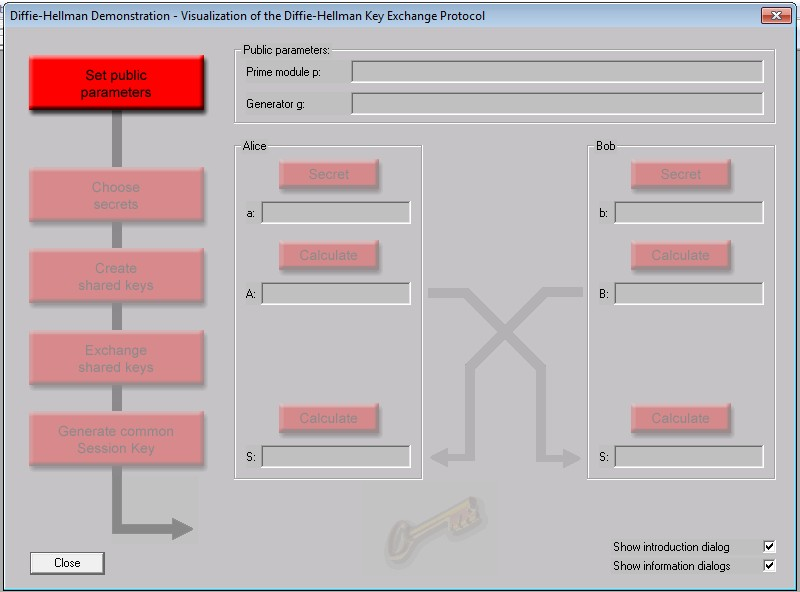
\includegraphics[width=\textwidth]{img/S001.jpg}
            \caption{Утилита демонстрации протокола Диффи-Хеллмана}%
            \label{img:a:1}
        \end{figure}
        \FloatBarrier{}

    \item Сгенерированы параметры $p$ (целое число) и $g$ (генератор --- натуральное число, не взаимно простое с $p$)

        \texttt{p = 164 459 422 689 066 243 011 729 968 057 438 442 455 606 356 397 837 044 700 733 361 991 165 383 163 799};\\
        \texttt{g = 90 781 356 746 102 774 580 779 638 749 722 545 280 765 577 832 398 664 019 008 562 895 851 301 528 787}

        $p$ и $g$ известны всем.

    \item Сгенерированы секреты:
        \texttt{a = 34 596 549 621 750 295 858 653 977 034 480 662 835 051 928 581 964 288 778 519 325 445 061 945 869 844};\\
        \texttt{b = 54 016 829 575 119 166 230 209 367 614 889 841 297 334 189 509 706 697 680 060 831 553 422 514 175 088}

        $a$ --- секрет Алисы, $b$ --- секрет Боба. Требования к секретам: $1 < a < p$, $1 < b < p$.

    \item Вычислены обшие ключи:
        \[ A = g^a \bmod p; B = g^b \bmod p \]
        \texttt{A = 34 467 817 907 976 045 230 452 302 928 382 669 365 886 312 181 386 385 984 225 792 489 434 184 933 013};\\
        \texttt{B = 142 731 903 542 858 044 148 169 623 036 564 507 677 299 220 545 763 907 701 621 198 404 943 777 173 031} 

    \item Произведен обмен ключами: Боб получает $A$, Алиса --- $B$.
    \item Стороны вычисляют сессионный ключ.
        \[ S = B^a \bmod p = {(g^b)}^a \bmod p = {(g^a)}^b \bmod p = A^b \bmod p \] 
        Таким образом, на обеих сторонах получается общий ключ.

        \texttt{S = 63 200 196 764 079 390 461 001 096 815 969 006 477 048 291 593 113 196 450 925 629 549 919 736 524 995}

        На рис.~\ref{img:a:2} представлены результаты работы
        \begin{figure}[h]
            \centering
            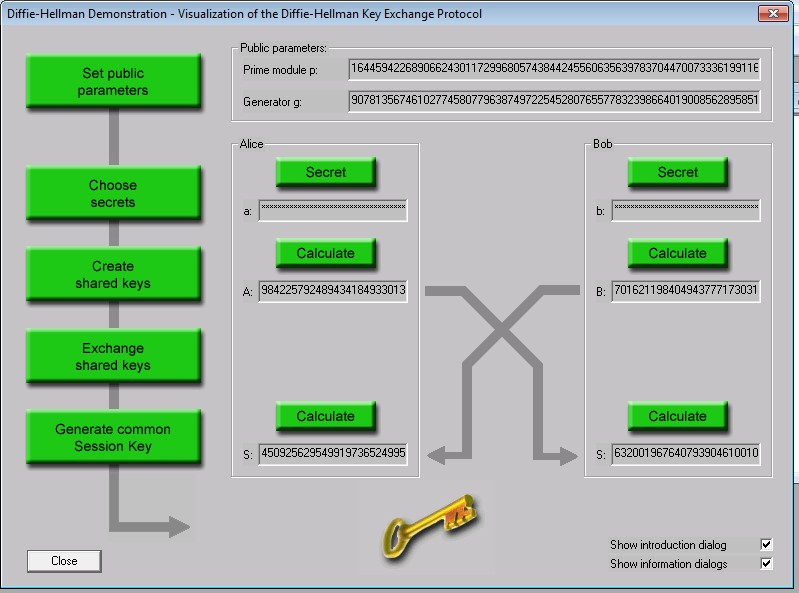
\includegraphics[width=\textwidth]{img/S002.jpg}
            \caption{Результаты работы}%
            \label{img:a:2}
        \end{figure}

        Логи работы в приложении А.

\end{enumerate}

\section{Шифр RSA}
\subsection{Описание шифра}
\begin{enumerate}
    \item Вычисление ключей:
        \begin{enumerate}
            \item Генерация двух больших простых чисел $p, q$ (держатся в секрете)
            \item $n = p \bullet q$
            \item Выбор взаимо просто $e < n$, взаимно простого с $\varphi(n)$\\
                $\varphi(n)$ --- функция Эйлера:
                \[ \varphi(p) = p - 1; \varphi(p^n) = p^n - p^{n-1}, \]
                если $p$ --- простое число,
                \[ \varphi(a) = \varphi(p_1^{n_1}) \ldots \varphi(p_k^{n_k}), \]
                если $a = p_1^{n_1} \ldots p_k^{n_k}$ --- натуральное число.
            \item Вычисление $d$ из $e \bullet d = 1 \bmod \varphi(n)$
            \item $(e,n)$ --- открытый ключ, $d$ --- закрытый ключ
        \end{enumerate}
    \item Шифрование:
        \begin{enumerate}
            \item Открытый текст разбивается на блоки $m_i: m_i < n$
            \item Каждый блок открытого текста преобразуется в шифротекст по формуле:
                \[ c_i = m_i^e \bmod n \]
        \end{enumerate}
    \item Расшифровка:
        \begin{enumerate}
            \item Шифротекст разбивается на блоки $c_i: c_i < n$
            \item Каждый блок шифротекста преобразуется в открытый текст по формуле:
                \[ c_i^d \bmod n \]
        \end{enumerate}
\end{enumerate}
\begin{figure}[h]
    \centering
    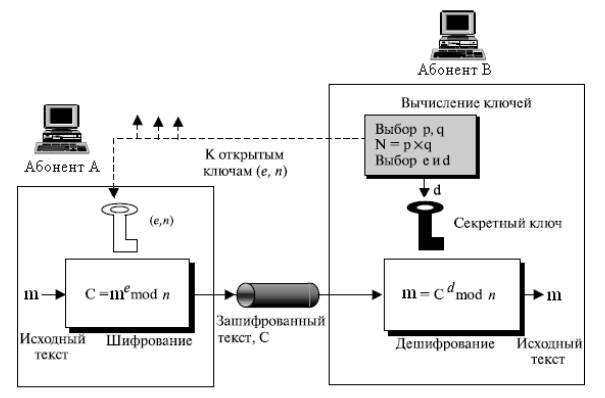
\includegraphics[width=0.5\textwidth]{img/S003.jpg}
    \caption{Иллюстрация работы шифра RSA}%
    \label{img:b:1}
\end{figure}

\FloatBarrier{}
\subsection{Формулировка задания}
\begin{enumerate}
    \item Запустите Demonstration утилиту Indiv.Procedures->RSACryptosystem->RSA Demonstration
    \item  Задайте в качестве обрабатываемого сообщения свою Ф.И.О.
    \item  Сгенерируйте открытый и закрытый ключи.
    \item  Зашифруйте сообщение. Сохраните скриншот результата.
    \item  Расшифруйте сообщение. Сохраните скриншот результата.
    \item Убедитесь, что расшифрование произошло корректно.
\end{enumerate}

\subsection{Выполнение задания}
\begin{itemize}
    \item Запущена демонстрационная утилита. Скриншот представлен на рис.~\ref{img:b:2}
    \begin{figure}[h]
        \centering
        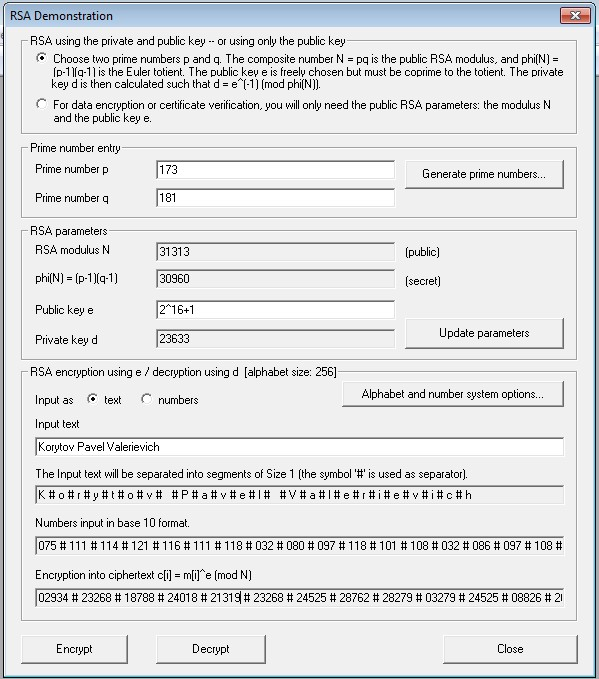
\includegraphics[width=\textwidth]{img/S004.jpg}
        \caption{Вид утилиты RSA Demonstration}%
        \label{img:b:2}
    \end{figure}
    
    \FloatBarrier{}
    \item Сгенерированы небольшие простые числа:
        \[ p = 173, q = 181 \] 
        Проведены вычисления
        \[ n = p \bullet q = 31313 \]
        \[ \varphi(n) = (p-1)(q-1) = 30960 \]
        \[ e = 2^{16} + 1 \]
        \[ d = 23633 \] 
    \item Произведено зашифрование текста \texttt{Korytov Pavel Valerievich}.

        Шифротекст: \texttt{02934 \# 23268 \# 18788 \# 24018 \# 21319 \# 23268 \# 24525 \# 28762 \# 28279 \# 03279 \# 24525 \# 08826 \# 20029 \# 28762 \# 18711 \# 03279 \# 20029 \# 08826 \# 18788 \# 07910 \# 08826 \# 24525 \# 07910 \# 20607 \# 14422}\\
    ``\#'' --- разделитель.
    
    \item Произведено расшифрование. Результат: \texttt{Korytov Pavel Valerievich} --- совпадает с исходным текстом.
\end{itemize}

\section{Исследование шифра RSA}
\subsection{Формулировка задания}
\begin{enumerate}
    \item 1. Выбрать текст на английском языке (не менее 1000 знаков) и сохранить в файле формата *.txt
    \item  Сгенерировать пары ассиметричных RSA-ключей утилитой Digital Signatures->PKI->Generate/Import Keys с различными длинами (4 варианта).
    \item  Зашифровать текст (примерно 1000 символов) различными открытыми ключами. Зафиксировать время зашифровки.
    \item  Расшифровать текст различными закрытыми ключами. Зафиксировать время зашифровки.
    \item  Проверить корректность расшифровки. Зафиксировать скриншоты результата.
\end{enumerate}

\subsection{Выполнение задания}
\begin{enumerate}
    \item Выбран текст на английском языке.

    \item Сгенерированы пары ассиметричных ключей с длинами 512, 768, 1024, 2048 бит.
    \begin{figure}[h]
        \centering
        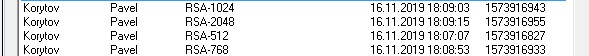
\includegraphics[width=\textwidth]{img/S005.jpg}
        \caption{Сгенерированные пары}%
        \label{img:c:1}
    \end{figure}
    
    \item Произведено зашифрование и расшифрование одного текста парами с разной длиной.
    \begin{figure}[h]
        \centering
        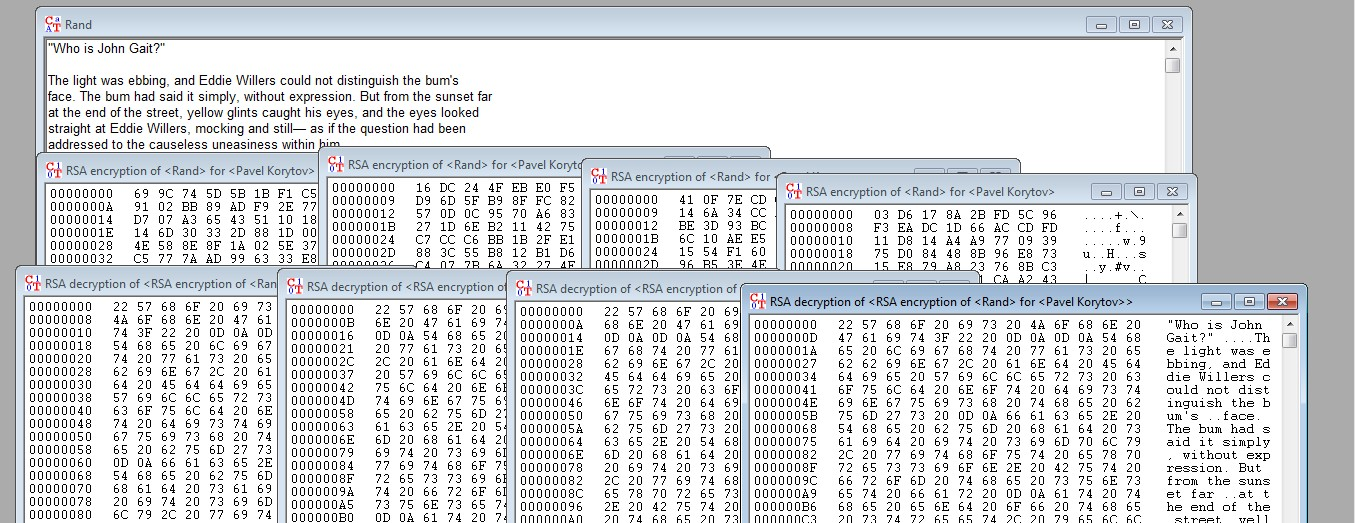
\includegraphics[width=\textwidth]{img/S006.jpg}
        \caption{Результаты шифрования и дешифрования}%
        \label{img:c:2}
    \end{figure}
    
    \FloatBarrier{}
    \begin{table}[h]
    \centering
    \begin{tabular}{@{}lll@{}}
    \toprule
    \textbf{Длина ключа (бит)} & \textbf{Время зашфирования (с)} & \textbf{Время расшифрования (с)} \\ \midrule
    512                        & 0.015                           & 0.109                            \\
    768                        & 0.016                           & 0.168                            \\
    1024                       & 0.014                           & 0.312                            \\
    2048                       & 0.031                           & 1.063                            \\ \bottomrule
    \end{tabular}
    \end{table}
\end{enumerate}

\section{Атака грубой силы на RSA}
\subsection{Формулировка задания}
\begin{enumerate}
    \item Запустите утилиту Indiv.Procedures->RSACryptosystem->RSA Demonstration
    \item Установите переключатель в режим «Choose two prime…».
    \item Выберите параметры $p$ и $q$ так, чтобы $n=pq> 256$.
    \item Задайте открытый ключ $e$.
    \item Зашифруйте произвольное сообщение и передайте его вместе с $n$ и $e$ коллеге. В ответ получите аналогичные данные от коллеги.
    \item Запустите утилиту Indiv.Procedures->RSACryptosystem->RSA Demonstration и установите переключатель в режим «For data encryption…»
    \item Выполните факторизацию модуля n командой Factorize…
    \item Используйте полученный результат для расшифровки сообщения полученного от коллеги. Проверьте корректность.
\end{enumerate}
\subsection{Выполнение задания}
\begin{enumerate}
    \item Произведено зашифрование сообщения:\\
    I shall choose friends among men, but neither slaves nor masters. And I shall choose only such as please me, and them I shall love and respect, but neither command nor obey. And we shall join our hands when we wish, or walk alone when we so desire.
    \[ p = 131, q = 211 \Rightarrow n = 27641 \]
    \[ e = 11 \]
    Сообщение передано коллеге.
    \item Получено сообщение:\\
    \texttt{22927 \# 09646 \# 29122 \# 09646 \# 29122 \# 25690 \# 09646 \# 04892 \# 30548 \# 23971 \# 25721 \# 12139 \# 13191 \# 30548 \# 28919 \# 24345 \# 23971 \# 28919 \# 30548 \# 28919 \# 24345 \# 09646 \# 30548 \# 12139 \# 29122 \# 23971 \# 25721 \# 25721 \# 09646 \# 12139 \# 28919 \# 30548 \# 29122 \# 09676 \# 20616 \# 13191 \# 04892 \# 09676 \# 28919 \# 21239 \# 30548 \# 13191 \# 20616 \# 30548 \# 09646 \# 23971 \# 04892 \# 28919 \# 24345 \# 30548 \# 09676 \# 12139 \# 30548 \# 28919 \# 24345 \# 09646 \# 30548 \# 09676 \# 20616 \# 24491 \# 09676 \# 31396 \# 09676 \# 24491 \# 20776 \# 23971 \# 25721 \# 03022 \# 30548 \# 14895 \# 24345 \# 13191 \# 12139 \# 09646 \# 30548 \# 22172 \# 24345 \# 13191 \# 30548 \# 24491 \# 09646 \# 20616 \# 21239 \# 30548 \# 09676 \# 20616 \# 24491 \# 09676 \# 31396 \# 09676 \# 24491 \# 20776 \# 23971 \# 25721 \# 30548 \# 04892 \# 09676 \# 27523 \# 24345 \# 28919 \# 12139 \# 26239 \# 30548 \# 03072 \# 23971 \# 20616 \# 20616 \# 13191 \# 28919 \# 30548 \# 03072 \# 25721 \# 23971 \# 09676 \# 29122 \# 30548 \# 28919 \# 13191 \# 30548 \# 25690 \# 09646 \# 30548 \# 24491 \# 09646 \# 18680 \# 09646 \# 20616 \# 24491 \# 09646 \# 04892 \# 12139 \# 30548 \# 13191 \# 18680 \# 30548 \# 29122 \# 09676 \# 20616 \# 13191 \# 04892 \# 09676 \# 28919 \# 09676 \# 09646 \# 12139 \# 03022}
    \[ n = 32111, e = 5 \]
    \item Проведена факторизация $n$: $n = 163 \bullet 197$. Произведено дешифрование:\\
    Remember also that the smallest minority on earth is the individual. Those who deny individual rights, cannot claim to be defenders of minorities.

\end{enumerate}

\section{Имитация атаки на гибридную криптосистему}
\section{Описание атаки}
Шифрование в гибридной модели осуществляется следующим образом:
\begin{enumerate}
    \item  Сообщение шифруется симметричным секретным ключом.
    \item  Секретный ключ шифруется открытым ключом.
    \item  Зашифрованное сообщение и ключ составляют цифровой конверт, который отправляется получателю.
    \item  Получатель сначала расшифровывает секретный ключ, затем расшифровывает секретным ключом шифротекст сообщения.
\end{enumerate}

Для атаки злоумышленник перехватывает цифровой конверт с зашифровнным сообщением и зашифрованным секретным ключом. 

\subsection{Формулировка задания}
\begin{enumerate}
    \item Подготовьте текст передаваемого сообщения на английском с вашим именем в конце.
    \item Запустите утилиту Analysis->Asymmetric Encr…->Side-Channel attack on «Textbook RSA»…
    \item Настройте сервер, указав в качестве ключевого слова ваше имя, используемое в конце текста.
    \item Выполните последовательно все шаги протокола.
    \item Сохраните лог-файлы участников протокола для отчета.
\end{enumerate}

\subsection{Выполнение задания}
\begin{enumerate}
    \item Подготовлен текст на английском языке
    \begin{figure}[h]
        \centering
        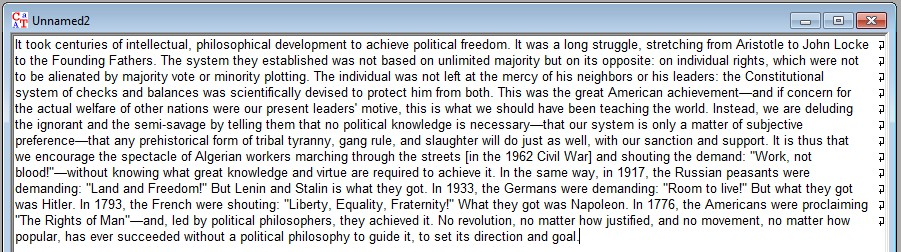
\includegraphics[width=\textwidth]{img/S007.jpg}
        \caption{Исходный текст}%
        \label{img:e:1}
    \end{figure}
    \FloatBarrier{}
    \item Проведена демонстрация атаки с помощью указанной утилиты
    \begin{figure}[h]
        \centering
        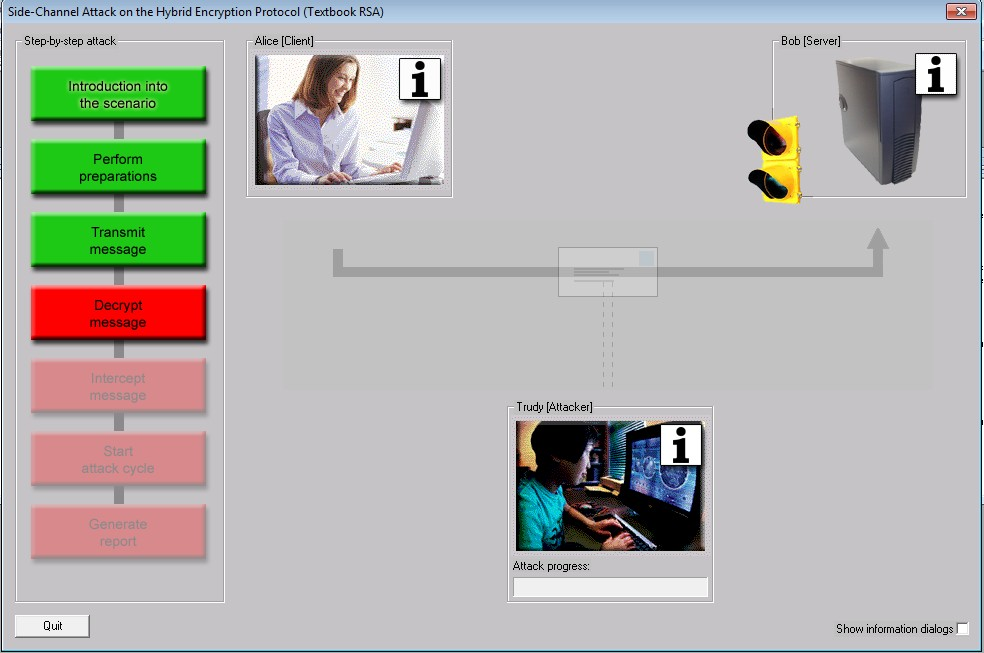
\includegraphics[width=\textwidth]{img/S010.jpg}
        \caption{Вид утилиты}%
        \label{img:e:4}
    \end{figure}
    \begin{figure}[h]
        \centering
        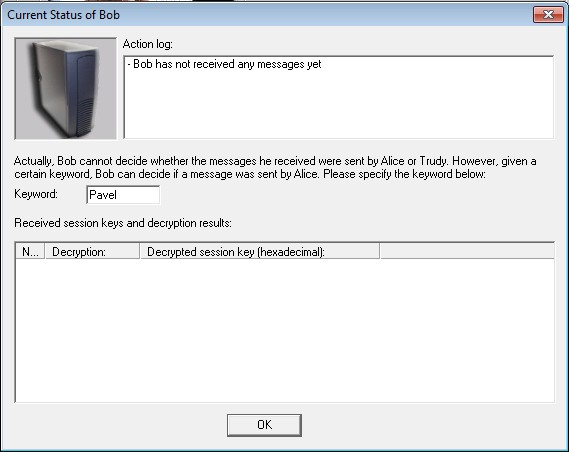
\includegraphics[width=\textwidth]{img/S008.jpg}
        \caption{Настройка ``сервера''}%
        \label{img:e:2}
    \end{figure}
    
    \begin{figure}[h]
        \centering
        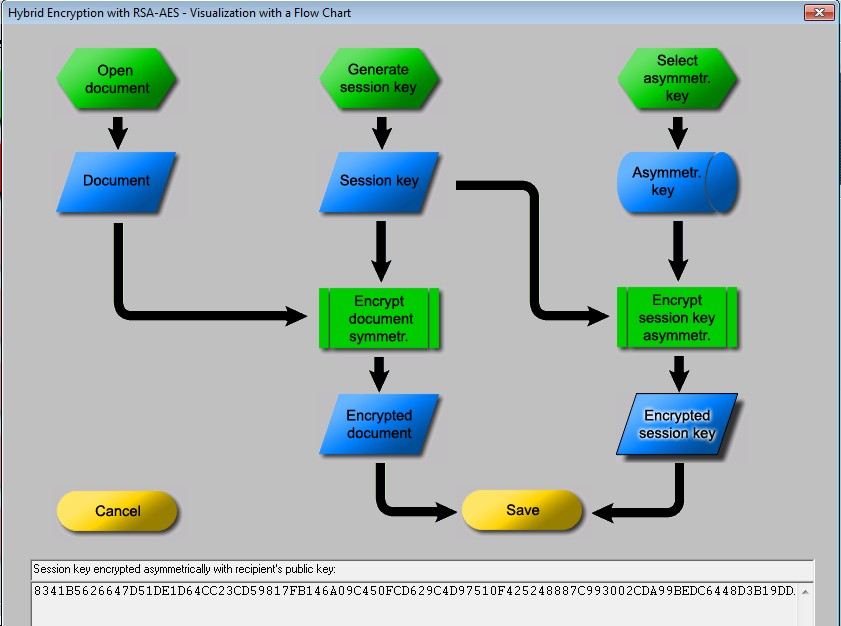
\includegraphics[width=\textwidth]{img/S009.jpg}
        \caption{Работа гибридной схемы}%
        \label{img:e:3}
    \end{figure}
    
    \begin{figure}[h]
        \centering
        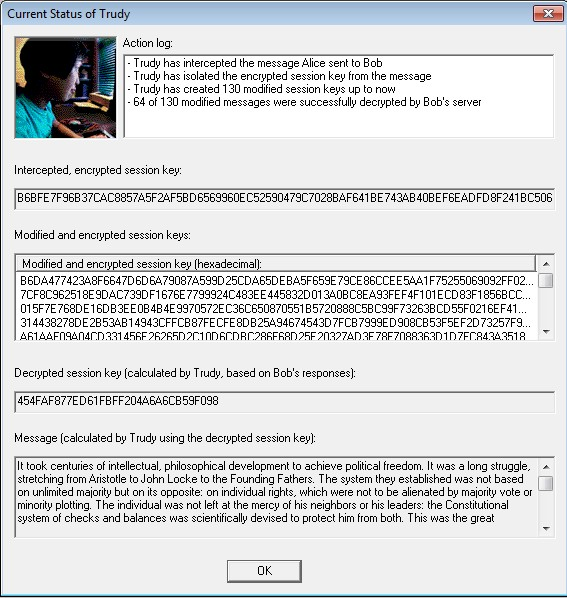
\includegraphics[width=\textwidth]{img/S011.jpg}
        \caption{Результаты атаки}%
        \label{img:e:4}
    \end{figure}
    Лог атаки в Приложении Б.
    
\end{enumerate}

\section{Выводы}
Исследован протокол Диффи-Хеллмана и ассиметричный шифр RSA.\@

Протокол Диффи-Хеллмана позволяет двум пользователям создать общий сеансовый ключ без обмена секретными ключами, чтобы обмениваться сообщениями по незащищенному каналу. Недостаток протокола --- уязвимость к атаке Man-In-The-Middle.

RSA --- асимметричный блочный шифр. Длины ключей --- 512, 768, 1024, 2048 бит, но 512 и 768 в настоящее время считаются недостаточными. 

Криптостойкость алгоритма основана на вычислительно сложной задаче факторизации числа.

Недостаток алгоритма --- относительно долгое время работы. Для компенсации этого недостатка используются гибридные системы --- асимметричный шифр используется для передачи ключа симметричного шифрования.

Атака на гибридную систему основана на многократной модификации перехваченного сообщения; она позволяет восстановить сеансовый ключ, но не закрытый ключ получателя.

\clearpage
\StartAddons{}
\section*{Приложение А}
\addonsubheader{Логи протокола Диффи-Хеллмана}
{\small
\lstinputlisting[]{./logs/log1.txt}
}

\clearpage
\section*{Приложение Б}
\addonsubheader{Логи Side Channel Attack}
{\small
\lstinputlisting[]{./logs/log2.txt}
}
\end{document}
